\newpage
\section{Картотека пациентов}

В \tmis ~для каждого пациента заводится регистрационная карточка, которая содержит всю персональную информацию о пациенте. Она регистрируется в системе при первом обращении пациента в МУ и выполняет функцию амбулаторной карты пациента. При всех последующих обращениях осуществляется поиск ранее зарегистрированной карточки пациента и привязка к ней очередного случая обращения. В случае изменения каких-либо персональных данных пациента, регистрационную карточку можно отредактировать. 

Таким образом, при работе с \tmis~персональные данные пациента вносятся в систему один раз, а медицинские записи добавляются при каждом обращении. Благодаря данному механизму значительно упрощается процесс получение врачом медицинской информации о предыдущих случаях обращения пациента.

Совокупность регистрационных карточек пациентов, случаев их обращений в ЛПУ и результатов обращений называется картотекой пациентов. Для доступа к картотеке пациентов необходимо нажать кнопку \btn{Обслуживание пациентов} на панели управления вверху страницы, либо нажать на блок \dm{Обслуживание пациентов} на главной странице системы (Рисунок \ref{img_gen_main}). Будет осуществлен переход на страницу \dm{Обслуживание пациентов} (Рисунок \ref{img_cl_find}). Здесь можно найти карточку пациента или зарегистрировать нового пациента, просмотреть предварительные записи на прием и данные обращений пациента, а так же зарегистрировать новые.

\begin{figure}[ht]\centering
 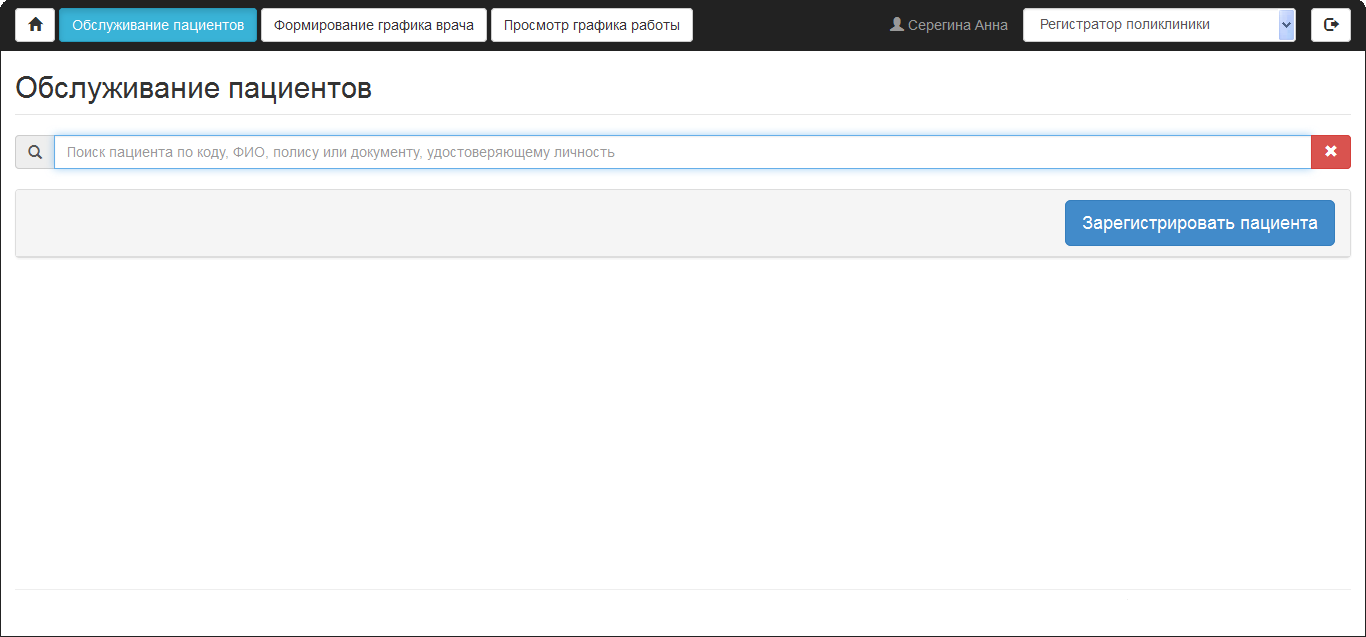
\includegraphics[width = 1\textwidth ,keepaspectratio]{cl_find}
 \caption{Страница поиска и обслуживания пациентов}
 \label{img_cl_find}
\end{figure} 

\subsection{Поиск регистрационной карточки пациента} \label{cl_find}

В верхней части страницы  \dm{Обслуживание пациентов} (Рисунок \ref{img_cl_find}) находится поле для задания параметров поиска пациентов. В него в произвольном порядке можно ввести фамилию, имя, отчество, дату рождения, код пациента, номера его полиса ОМС или документа, удостоверяющего личность. Дату рождения в поле поиска можно вводить в формате <<ДД.ММ.ГГГГ>> либо <<ДДММГГГГ>> без разделителей. 

После ввода всех необходимых критериев поиска, следует нажать клавишу \keys{Enter} на клавиатуре либо кнопку \btn{Найти} в правой части поля поиска. После непродолжительного ожидания на экране появится список найденных согласно заданным условиям пациентов (Рисунок \ref{img_cl_findrez}). 
 
\begin{figure}[ht]\centering
 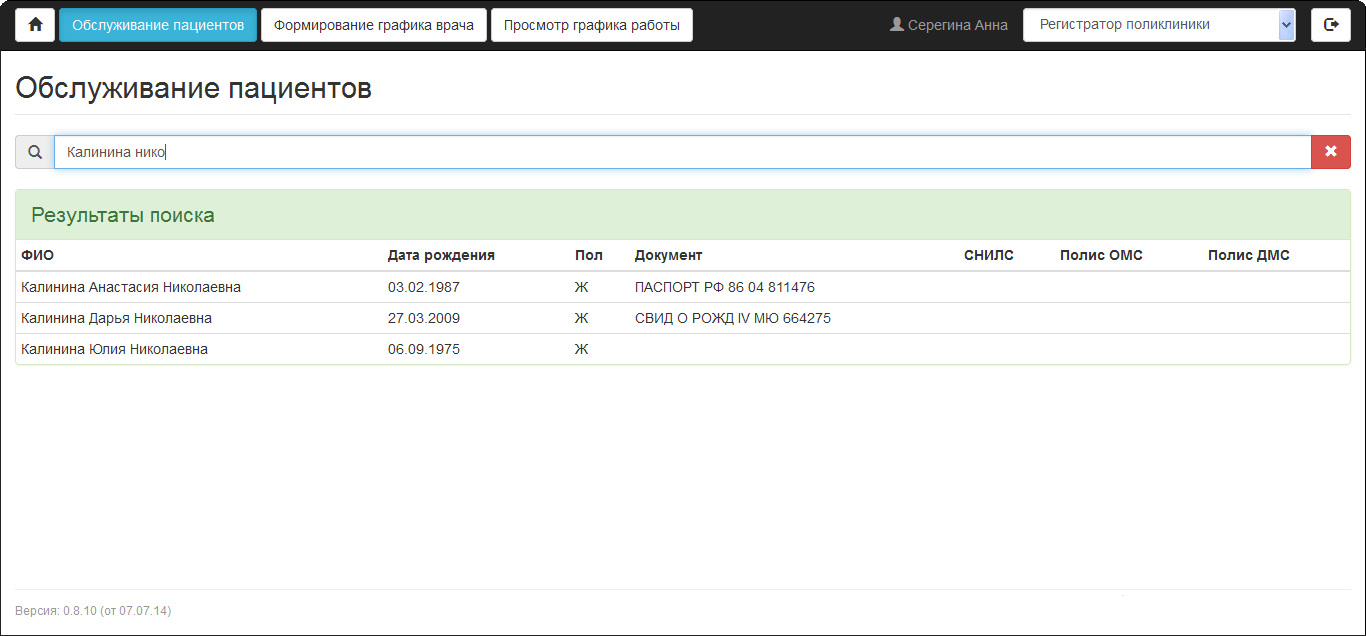
\includegraphics[width = 1\textwidth ,keepaspectratio]{cl_findrez}
 \caption{Результаты поиска пациентов}
 \label{img_cl_findrez}
\end{figure} 

Если по заданным параметрам не будет найдено ни одного пациента, по под полем поиска появится сообщение <<Пациент не найден в базе данных>>.

\ifthenelse{\isnamedefined{fullversion} \OR \isnamedefined{regversion}}
{
\subsection{Регистрационная карточка пациента} \label{cl_card}

Регистрационная карточка пациента содержит всю персональную информацию о пациенте: его фамилию, имя, отчество, дату рождения, адрес, сведения о документах пациента, его страховых полисах, льготах, занятости и т.д. Вся эта информация должна вводиться регистратором с первичных документов пациента при его первом обращении в ЛПУ. В момент регистрации пациента ему присваивается уникальный код, по которому его регистрационную карточку можно быстро найти в картотеке пациентов.

Для регистрации нового пациента необходимо нажать  кнопку \btn{Зарегистрировать пациента} на странице обслуживания пациентов (Рисунок \ref{img_cl_find}). Откроется страница регистрационной карточки пациента (Рисунок \ref{img_cl_card}). 

\begin{figure}[!ht]\centering
 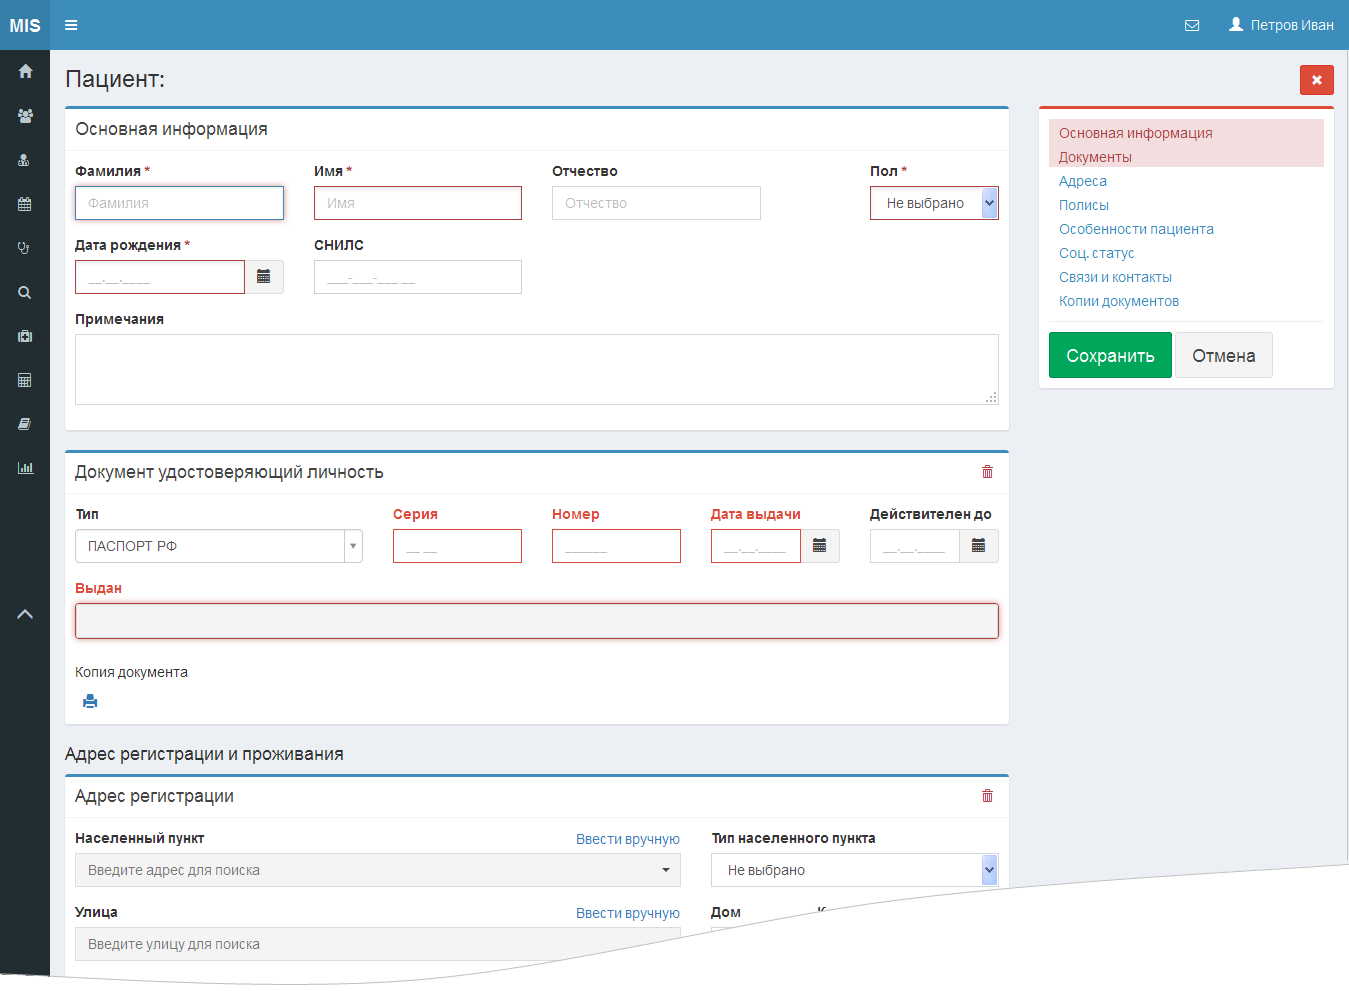
\includegraphics[width = 1\textwidth ,keepaspectratio]{cl_card}
 \caption{Регистрационная карточка пациента}
 \label{img_cl_card}
\end{figure} 

Карточка содержит большое количество информации. Для удобства пользователя, информация разбита на логические блоки. Для перехода к определенному блоку можно щелкнуть левой кнопкой мыши по его названию в левой части страницы либо воспользоваться полосой прокрутки и найти раздел самостоятельно.  

\subsubsection{Блок <<Основная информация>>}

Поля \dm{Фамилия}, \dm{Имя}, \dm{Дата рождения} и \dm{Пол} в регистрационной карточке пациента являются обязательными для заполнения. Они помечены символом <<*>> красного цвета.

Дата рождения пациента может вводиться  с клавиатуры или выбираться из календаря (подрбнее см. раздел \ref{gen_cal}). При заполнении с клавиатуры нужно вводить дату в формате <<ДДММГГГГ>> или <<ДД.ММ.ГГГГ>>. Недостающие разделители вставляются автоматически. Аналогичным образом в \tmis заполняются все поля, содержащие даты.

Значение поля \dm{Пол} может вводиться с клавиатуры или выбираться из раскрывающегося списка. 

В поле \dm{СНИЛС} достаточно ввести только цифры, разделительные тире будут вставлены автоматически. При вводе СНИЛС автоматически проводится проверка корректности введенного значения. В случае, если введенное значение не прошло проверку, поле будет выделено красным цветом и справа от поля появится подсказка <<Введен невалидный СНИЛС>>. Сохранение карточки пациента с неверным СНИЛС невозможно.

В поле \dm{Примечание} можно внести дополнительные сведения о пациенте, для которых не предусмотрено отдельных полей в карточке пациента. 
 
\subsubsection{Блок <<Документ удостоверяющий личность>>}

В данном блоке (Рисунок \ref{img_cl_card}) указываются данные документа, удостоверяющего личность пациента. Как правило, для детей таким документом является свидетельство о рождении, а для взрослых – паспорт. Однако, возможны и другие варианты. 
\begin{itemize}
 \item \dm{Тип документа} выбирается из раскрывающегося списка. В зависимости от выбранного типа, определяется набор реквизитов документа, доступных и обязательных для  заполнения. Обязательные для заполнения поля подсвечиваются красным цветом. Для большинства типов документов обязательно требуется указать серию, номер, дату выдачи и кем был выдан документ. 
 \item \dm{Серия, Номер}. Для каждого типа документов задается собственный формат серии и номера: определяется их длина,  возможность ввода в поле буквенных значений, а так же других специальных символов. 
 \item В поле \dm{Дата выдачи} дата может вводиться с клавиатуры или выбираться из календаря (подробнее см. раздел \ref{gen_cal}) 
 \item Поле \dm{Действителен до} заполняется аналогично предыдущему. Если документ не имеет срока действия, то поле может оставаться пустым. Данное поле необходимо заполнить обязательно, если в \tmis~происходит изменение сведений о действующем документе, удостоверяющем личность (т.е. если пациент предоставил новый документ того же типа, что и предыдущий). 
 \item В поле \dm{Выдан} можно выбрать значение из справочника или ввести произвольный текст с клавиатуры. По мере ввода текста в данное поле, в его  раскрывающемся списке будет производиться фильтрация значений в соответствии с введенным текстом. Для выбора значения из справочника необходимо щелкнуть по нему левой кнопкой мыши или переместить на него курсор с помощью стрелок на клавиатуре, а затем нажать клавишу \keys{Enter}. Для сохранения значения не из справочника необходимо обязательно нажать клавишу \keys{Enter} в данном поле после завершения ввода. Для очистки поля нужно нажать кнопку 
\includegraphics[scale=0.6]{clear} в правой части поля.
\end{itemize}

После сохранения информации о документе, удостоверяющем личность пациента появляется возможность прикрепления скан-копии указанного документа (Рисунок \ref{img_cl_docs}). Для этого необходимо нажать кнопку \btn{Добавить копию документа} в нижней части данного блока и в появившемся всплывающем окне выполнить прикрепление документа со сканера или из файла (см. раздел \ref{cl_copydocs}).  

\begin{figure}[ht]\centering
 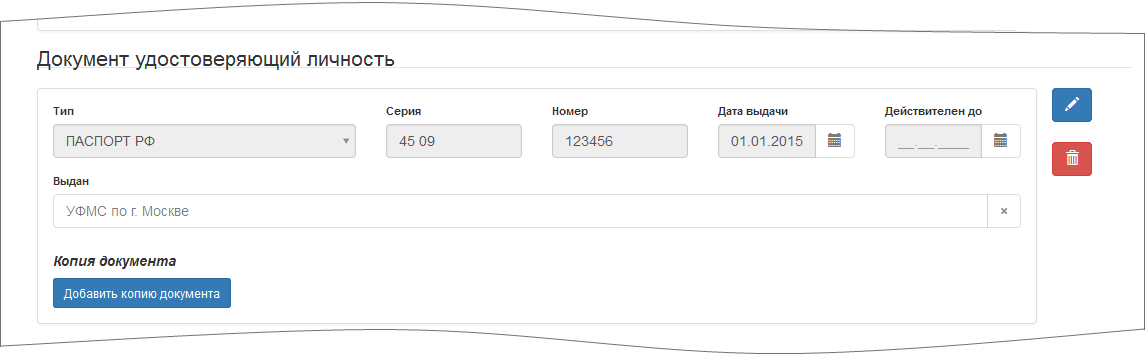
\includegraphics[width = 1\textwidth ,keepaspectratio]{cl_docs}
 \caption{Регистрационная карточка пациента. Блок ввода документа, удостоверяющего личность}
 \label{img_cl_docs}
\end{figure} 

\subsubsection{Блок <<Адрес регистрации и проживания>>}

В регистрационной карточке существует возможность указания двух адресов для каждого пациента: адреса регистрации и адреса фактического проживания (Рисунок \ref{img_cl_adres}). 

\begin{figure}[ht]\centering
 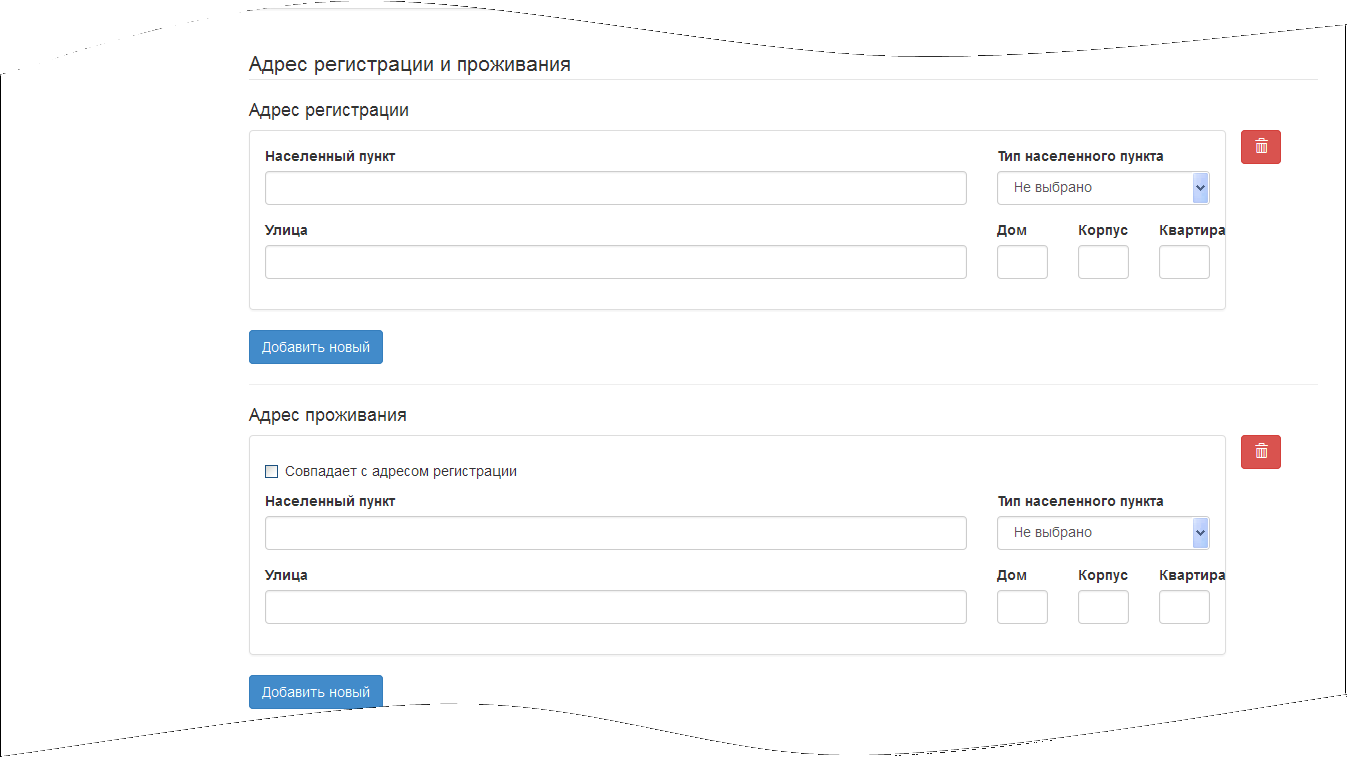
\includegraphics[width = 1\textwidth ,keepaspectratio]{cl_adres}
 \caption{Регистрационная карточка пациента. Блок ввода адреса регистрации.}
 \label{img_cl_adres}
\end{figure} 

Заполнение адреса рекомендуется выполнять с помощью всероссийского классификатора адресов -- КЛАДР. Для заполнения полей \dm{Населенный пункт} или \dm{Улица} нужно ввести его(ее) наименование или часть наименования в соответствующее поле и нажать клавишу \keys{Enter} на клавиатуре. В раскрывающемся списке поля появится перечень наименований, найденных в соответствии с условиями поиска. Необходимо выбрать из раскрывающегося списка требуемое значение, щелкнув по нему левой кнопкой мыши или установив на него курсор с помощью стрелок на клавиатуре и нажав клавишу \keys{Enter}. Поля \dm{Дом}, \dm{Корпус} и \dm{Квартира} могут заполняться произвольными значеними.

Если для данных, внесенных в поля \dm{Населенный пункт} и \dm{Улица}, не найдены соответствия в справочнике КЛАДР, то поля будут считаться заполненными с ошибками. Они будут подсвечены красным цветом, а в верхней части блока появится сообщение об ошибке <<Введенный адрес не найден в справочнике адресов Кладр. Ввести адрес вручную?>> (Рисунок \ref{img_cl_adrf}). Сохранение карточки пациента при этом будет невозможно. 

\begin{figure}[ht]\centering
 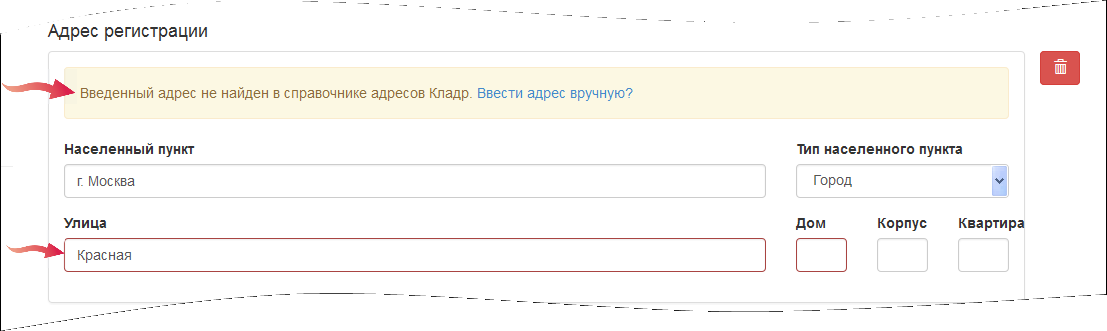
\includegraphics[width = 1\textwidth ,keepaspectratio]{cl_adrf}
 \caption{Регистрационная карточка пациента. Блок ввода адреса регистрации. Адрес не найден в справочнике КЛАДР}
 \label{img_cl_adrf}
\end{figure} 

В такой ситуации следует еще раз проверить правильность написания названий населенного пункта и улицы, попытаться использовать другое написание или альтернативные названия. Если и после этого найти соответствие в справочнике не удалось, можно щелкнуть левой кнопкой мыши по фразе <<Ввести адрес вручную?>> в тексте сообщения об ошибке. Поля  \dm{Населенный пункт}, \dm{Улица}, \dm{Дом}, \dm{Корпус} и \dm{Квартира} при этом станут недоступными для редактирования, но появится новое поле \dm{В свободном виде} в нижней части блока, куда можно будет ввести адрес в произвольной форме. Проверка на соответствие справочнику КЛАДР при этом производиться не будет (Рисунок \ref{img_cl_adrfree}). 

\begin{vnim}
Ввод адреса в свободной форме можно применять только в крайних случаях, если выбор из справочника КЛАДР абсолютно невозможен. 
\end{vnim}

\begin{figure}[ht]\centering
 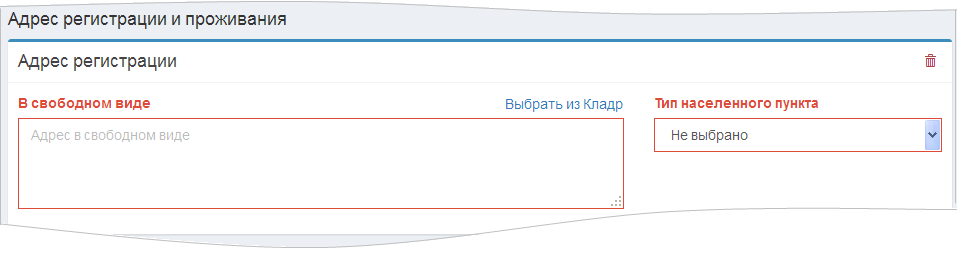
\includegraphics[width = 1\textwidth ,keepaspectratio]{cl_adrfree}
 \caption{Регистрационная карточка пациента. Блок ввода адреса регистрации. Ввод адреса в свободной форме}
 \label{img_cl_adrfree}
\end{figure}   

\begin{prim}
Для того, чтобы от свободного ввода снова вернуться к вводу адреса по справочнику КЛАДР, нужно щелкнуть в сообщении об ошибке вверху блока по фразе <<Выбрать из Кладр>>. При этом поле \dm{В свободном виде} исчезнет, а остальные поля снова станут доступны для редактирования.
\end{prim}

В полях ниже, аналогичным способом можно ввести адрес фактического проживания пациента. Если адрес фактического проживания совпадает с адресом регистрации, то в подразделе \dm{Адрес проживания} можно установить флажок \dm{Совпадает с адресом регистрации}. Тогда данные из подраздела \dm{Адрес регистрации} будут скопированы в соответствующие поля подраздела \dm{Адрес проживания}. Редактирование адреса проживания при этом становится недоступно. 
 
\subsubsection{Блок <<Медицинские полисы>>}
  
В подразделе \dm{Полис ОМС} (Рисунок \ref{img_cl_police}) указываются данные действующего полиса обязательного медицинского страхования. Необходимо указать тип полиса, его серию и номер, дату выдачи, срок действия и название СМО, выдавшей полис. Поле \dm{Действителен до} может оставаться незаполненным, если срок действия полиса не ограничен. Остальные поля являются обязательными для заполнения. 

В поле \dm{Страховая медицинская организация} можно выбрать наименование из справочника или ввести произвольное значение с клавиатуры. По мере ввода текста в данное поле, в его  раскрывающемся списке будет производиться фильтрация значений в соответствии с введенным текстом. Для выбора значения из справочника необходимо щелкнуть по нему левой кнопкой мыши или установить на него курсор с помощью стрелок на клавиатуре, а затем нажать клавишу \keys{Enter}. Для сохранения значения отсутствуюшего в справочнике требуется нажать клавишу \keys{Enter} в данном поле после завершения ввода. Для очистки поля нужно нажать кнопку 
\includegraphics[scale=0.6]{clear} в правой части поля.

\begin{figure}[ht]\centering
 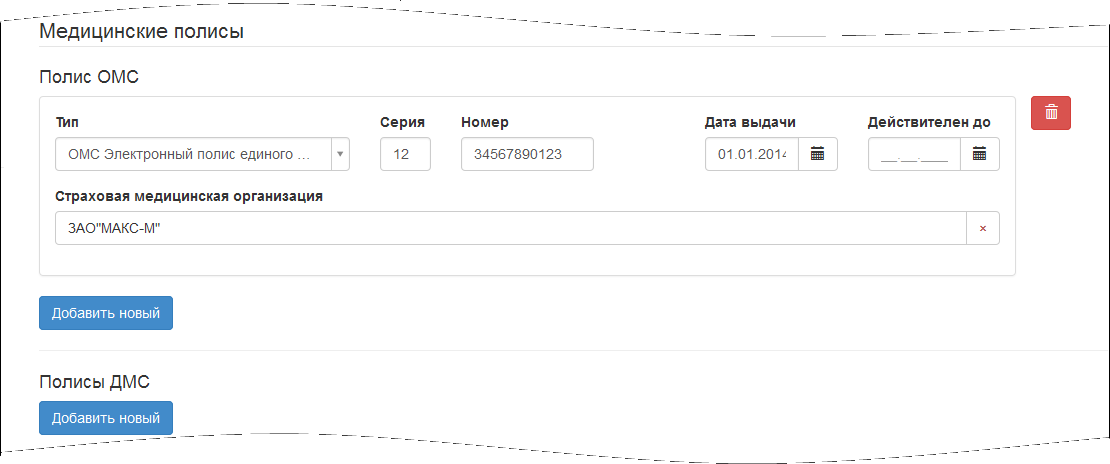
\includegraphics[width = 1\textwidth ,keepaspectratio]{cl_police}
 \caption{Регистрационная карточка пациента. Блок ввода полисов пациента.}
 \label{img_cl_police}
\end{figure}  

В подразделе \dm{Полис ДМС} по умолчанию поля скрыты. Для добавления полиса ДМС в карточку пациента необходимо нажать кнопку \btn{Добавить новый} в подразделе \dm{Полисы ДМС}. Появятся поля, аналогичные полям в подразделе \dm{Полис ОМС}. Заполнение данных полиса ДМС осуществляется аналогично заполнению раздела \dm{Полисы ОМС}.

Пациент может иметь только один действующий полис ОМС и любое количество действующих полисов ДМС. Поэтому при добавлении нового полиса ОМС, он заменяет ранее зарегистрированный. При добавлении нового полиса ДМС он добавляется к списку существующих полисов ДМС. 

\begin{prim}
При изменении данных полиса или документа, удостоверяющего личность, ранее введенные данные не теряются. Все ранее зарегистрированные для пациента полисы  и документы, удостоверяющие личность, можно найти в блоке \dm{История изменений документов} (см.раздел \ref{cl_docshistory})
\end{prim}

После сохранения данных полиса, можно прикрепить фотокопию данного документа к регистрационной карточке. Для этого необходимо нажать кнопку \btn{Добавить копию документа} в конце соответствуюшего подраздела и выполнить прикрепление документа со сканера либо из файла (см. раздел \ref{cl_copydocs})


\subsubsection{Блок <<Особенности пациента>>} 

Блок \dm{Особенности пациента} содержит жизненно-важные параметры, необходимые для оказания медицинской помощи (витальную информацию): группу крови, сведения об аллергии и медикаментозной непереносимости (Рисунок \ref{img_cl_osob}). 

\begin{figure}[!ht]\centering
 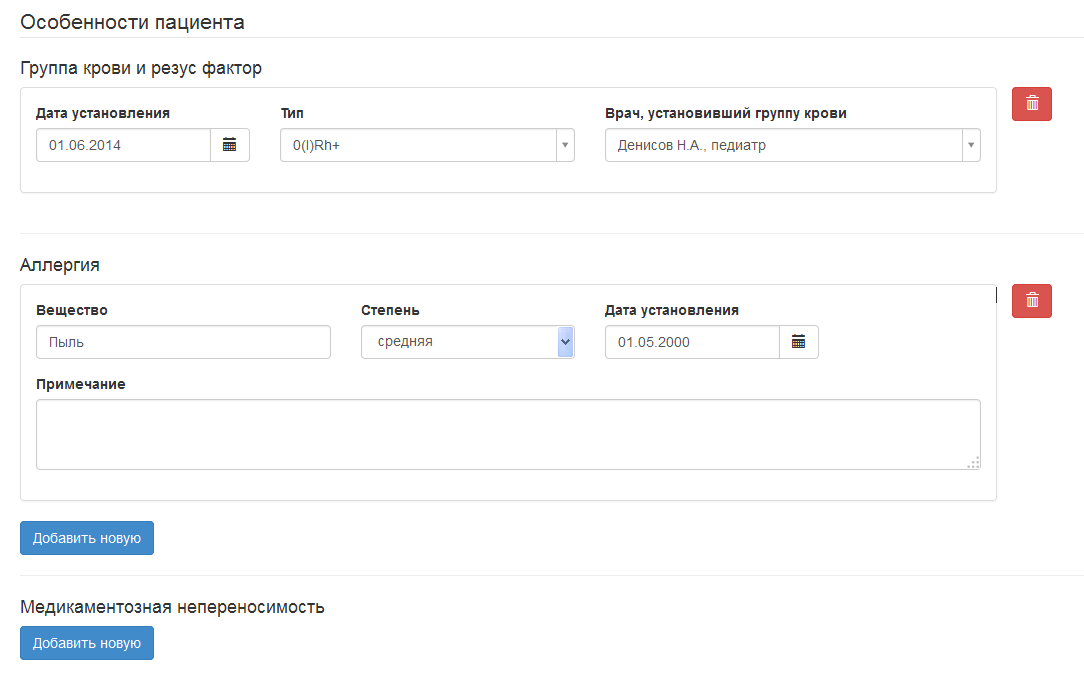
\includegraphics[width = 1\textwidth ,keepaspectratio]{cl_osob}
 \caption{Регистрационная карточка пациента. Блок <<Особенности пациента>>}
 \label{img_cl_osob}
\end{figure} 

Блок содержит 3 подраздела: 
\begin{itemize}
 \item Группа крови и резус фактор;
 \item Аллергия;
 \item Медикаментозная непереносимость.
\end{itemize}

По умолчанию поля для каждого из подразделов скрыты. Для добавления информации в какой-либо из подразделов нходимоеобходимо нажать кнопку \btn{Добавить новую}. Тогда на странице появятся дополнительные поля для ввода информации соответствующего подраздела.

В подразделе \dm{Группа крови и резус-фактор} хранится информация о группе крови  и резусе пациента. Если группа крови пациента известна, то ее необходимо внести в регистрационную карточку. Для этого следует нажать кнопку \btn{Добавить новую} и заполнить появившиеся поля. В поле \dm{Дата установления} нужно указать дату установления группы крови, в поле \dm{Тип} следует выбрать группу крови и резус-фактор из справочника, в поле \dm{Врач, установивший группу крови} выбрать фамилию врача из справочника сотрудников (по умолчанию указывается фамилия текущего пользователя). Все поля обязательны для заполнения. 

Если группа крови была установлена в другом МУ, то в качестве врача, установившего группу крови, следует указывать сотрудника, зарегистрировавшего ее в карточке пациента.

\begin{vnim}
Редактирование группы крови и резус-фактора после сохранения регистрационной карточки пациента становится невозможным. Проявите особую аккуратность при внесении этих данных.
\end{vnim}

Подразделы \dm{Аллергия} и \dm{Медикаментозная непереносимость} заполняются по одному и тому же принципу. В поле  \dm{Вещество (Препарат)} необходимо ввести описание аллергена, например <<пыль>> или <<ампициллин>>, в ячейке \dm{Степень} выбрать из списка степень аллергической реакции, в ячейке \dm{Дата установления} ввести дату установления аллергии (медикаментозной непереносимости), в поле \dm{Примечание}, можно указать дополнительные сведения относительно реакции. В каждом подразделе может содержаться любое количество записей. Добавление новых записей производится нажатием кнопки \btn{Добавить новую}. Поля \dm{Вещество (Препарат)}, \dm{Степень} и \dm{Дата установления} являются обязательными для заполнения. В случае их незаполнения, поля будут подсвечиваться красным цветом, сохранение регистрационной карточки пациента при этом будет невозможно.

\subsubsection{Блок <<Социальные статусы>>} 

В этом блоке можно внести ряд дополнительных сведений о пациенте, которые используются, в первую очередь для статистического учета (Рисунок \ref{img_cl_socst}): 
\begin{itemize}
 \item \dm{Инвалидность} -- данные о виде инвалидности пациента и документах, подтверждающих ее.
 \item \dm{Занятость} -- сведения о занятости пациента.
 \item \dm{Гражданство}.
\end{itemize}

По умолчанию поля для каждого из подразделов скрыты. Для добавления информации в какой-либо из подразделов необходимо нажать кнопку \btn{Добавить инвалидность}, \btn{Добавить занятость} или \btn{Добавить гражданство} соответственно.

\begin{figure}[ht]\centering
 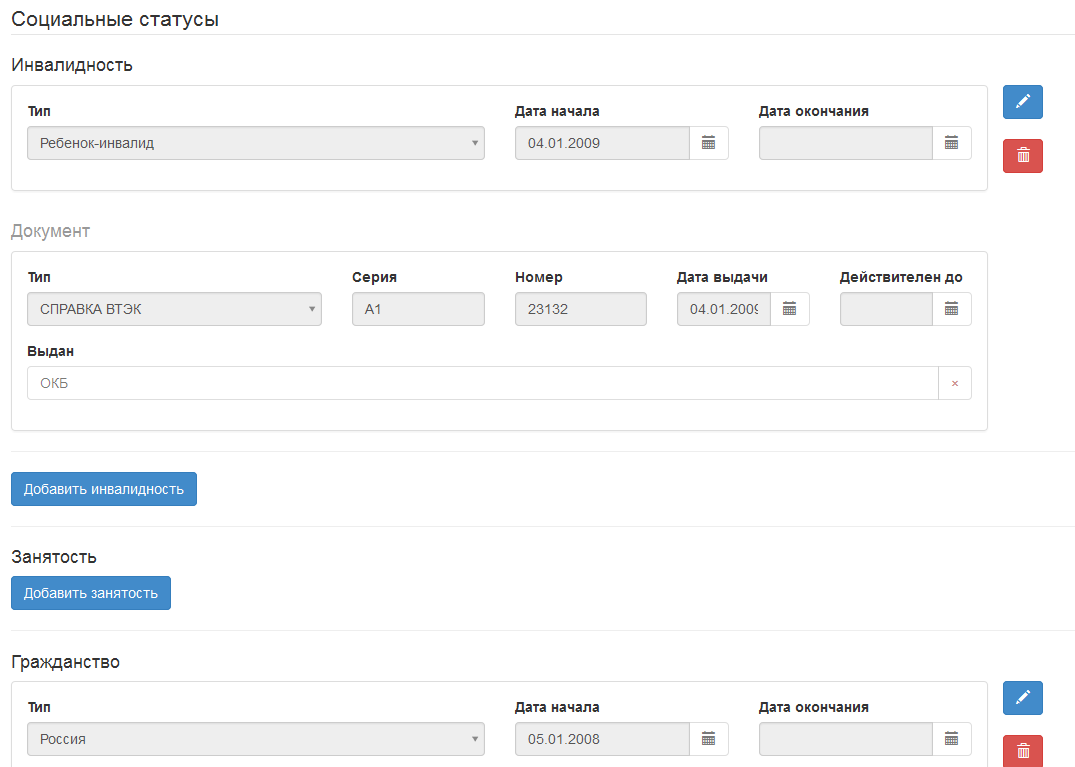
\includegraphics[width = 1\textwidth ,keepaspectratio]{cl_socst}
 \caption{Регистрационная карточка пациента. Блок <<Социальные статусы>>}
 \label{img_cl_socst}
\end{figure} 

При заполнении данных перечисленных подразделов необходимо выбрать значение в поле \dm{Тип} и указать дату в поле \dm{Дата начала}. Если настоящая дата установления статуса (например, гражданства) неизвестна, то можно указать текущую дату. Для инвалидности обязательно следует указывать настоящую дату установления в поле \dm{Дата начала}, а так же ввести данные документа, подтверждающего инвалидность.


\begin{prim}
Данные обо всех документах, подтверждающих инвалидность можно так же просмотреть в блоке \dm{История изменений документов} (см. раздел \ref{cl_docshistory}).
\end{prim}
 
\subsubsection{Блок <<Контактная информация и родственники>>}

В подраздел \dm{Связи с другими пациентами} содержит указатели на регистрационные карточки родственников пациента (Рисунок \ref{img_cl_contact}). 

\begin{vnim}
Для создания связи родственник должен быть зарегистрирован в \tmis.
\end{vnim}

\begin{figure}[ht!]\centering
 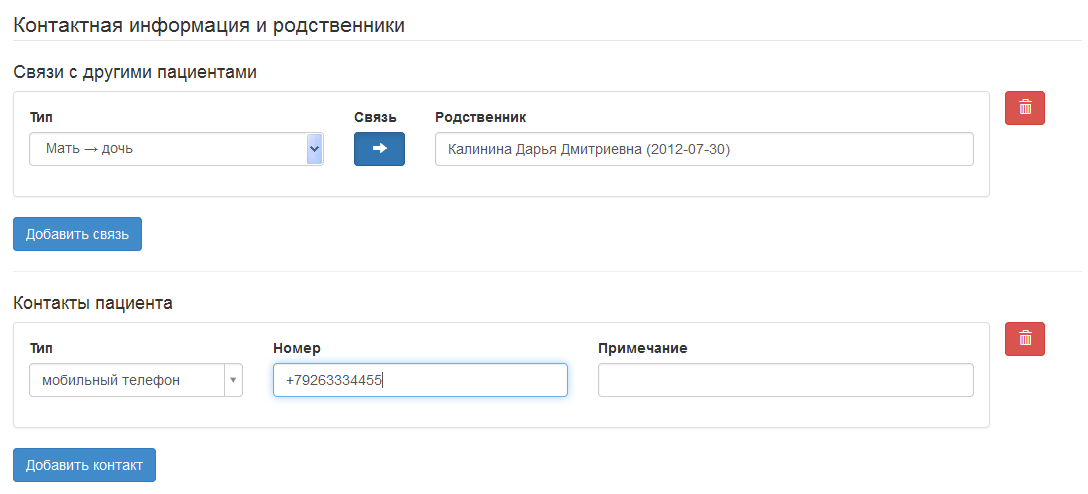
\includegraphics[width = 1\textwidth ,keepaspectratio]{cl_contact}
 \caption{Регистрационная карточка пациента. Блок <<Контактная информация и родственники>>}
 \label{img_cl_contact}
\end{figure} 

Для добавления связи необходимо нажать кнопку \btn{Добавить связь}, выбрать тип связи в поле \dm{Тип} и соответствующего пациента из БД в поле \dm{Родственник}. Список доступных значений в поле \dm{Тип} определяется значением в поле \dm{Пол} для текущего пациента, а так же направлением стрелки в поле \dm{Связь}. Для изменения направления связи необходимо щелкнуть по кнопке с изображением стрелки в поле \dm{Связь}. Для поиска родственника необходимо ввести его фамилию в поле \dm{Родственник}. По мере набора фамилии будет осуществляться поиск пациентов в БД. Результат поиска будет отображаться в раскрывающемся списке поля. Следует выбрать из этого списка нужного пациента. Если не будет найдено соответствия введенных данных с пациентами в БД, поле \dm{Родственник} будет подсвечено красным цветом. Сохранение регистрационной карточки пациента при этом будет невозможно.

Возможен ввод нескольких родственников в карточку пациента. Для добавления нового родственника следует нажать кнопку \btn{Добавить связь} и внести данные во вновь открывшиеся поля.

В подразделе \dm{Контакты пациента} можно хранить контактные данные пациента: номера телефонов, факсов, данные контактных лиц, адреса электронной почты и т.п.

Для добавления контактной информации следует нажать кнопку \dm{Добавить контакт}, затем во вновь открывшиеся поля ввести следующие данные: в поле \dm{Тип} выбрать тип контактной информации, в поле \dm{Номер} ввести номер телефона, факса, адрес электронной почты, в поле \dm{Примечание} можно указать любую дополнительную информацию относительно контакта, например, имена родственников, рекомендуемое время звонка и т.д.

Возможен ввод нескольких контактов в карточку пациента. Для добавления нового контакта следует нажать кнопку \btn{Добавить контакт} и внести данные во вновь открывшиеся поля.


\subsubsection{Копии документов} \label{cl_copydocs}

В данном блоке можно добавить или просмотреть фотокопии документов пациента, прикрепленные к карточке (Рисунок \ref{img_cl_copydocs}). 

\begin{figure}[ht!]\centering
 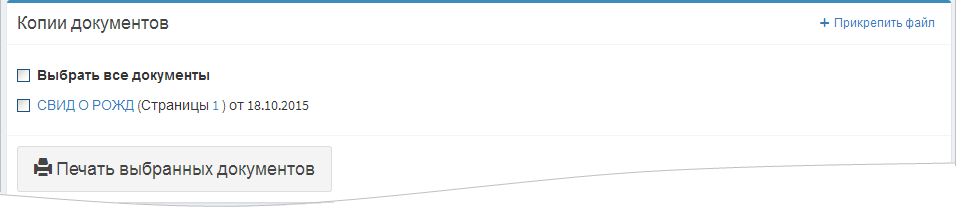
\includegraphics[width = 1\textwidth ,keepaspectratio]{cl_copydocs}
 \caption{Регистрационная карточка пациента. Блок <<Копии документов>>}
 \label{img_cl_copydocs}
\end{figure} 

Добавление копий документов может производиться как в данном блоке, так и в блоке, соответствующем типу сохраняемого документа. Для добавления документа из данного блока нужно нажать кнопку \btn{Прикрепить файл}. Для добавления копии документа из блока, соответствующего типу добавляемого документа,  необходимо нажать кнопку \btn{Добавить копию документа} в конце соответствующего типу документа раздела или блока. Данная кнопка доступна только после сохранения информации о документе пациента. После нажатия на кнопку появляется  всплывающее окно(Рисунок \ref{img_cl_addcopydoc}), где имеется возможность прикрепления копии документа непосредственно со сканера или из ранее сохраненного файла.

\begin{figure}[ht]\centering
 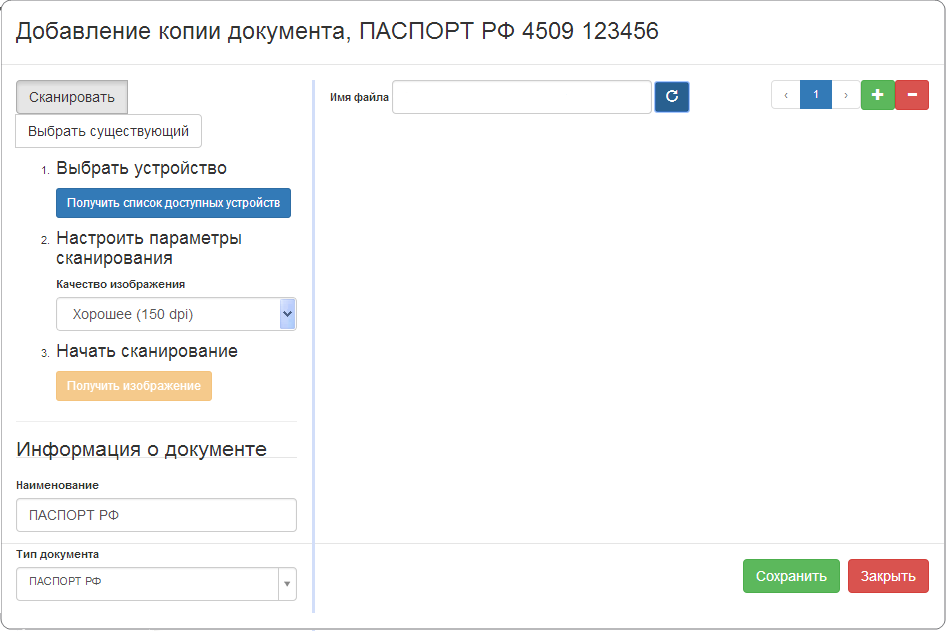
\includegraphics[width = 1\textwidth ,keepaspectratio]{cl_addcopydoc}
 \caption{Добавление копии документа со сканера}
 \label{img_cl_addcopydoc}
\end{figure} 

Для получения копии документа со сканера необходимо нажать <<Сканировать>> в левом верхнем углу окна (выбирается по умолчанию) (Рисунок \ref{img_cl_addcopydoc}). При отсутствии сканера в списке устройств в окне требуется нажать кнопку \btn{Получить список доступных устройств}. После непродолжительной обработки под кнопкой появится список устройств, подключения к которым обнаруженны на данном компьютере. Необходимо установить переключатель на устройство-сканер, выбрать качество сканирования в раскрывающемся списке ниже и нажать кнопку \btn{Получить избражение}. Начнется процесс сканирования, который может занять несколько секунд. После его завершения скан-копия документа появится в правой части всплывающего окна.

Для сохранения копии документа из файла необходимо нажать <<Выбрать существующий>> в левом верхнем углу окна. Далее следует нажать кнопку \btn{Выберите файл} и в появившемся окне указать путь к ранее сохраненной фотокопии документа. После загрузки файла в систему, он так же отобразится в правой части окна (Рисунок \ref{img_cl_addcopydoc2}).   

\begin{figure}[ht]\centering
 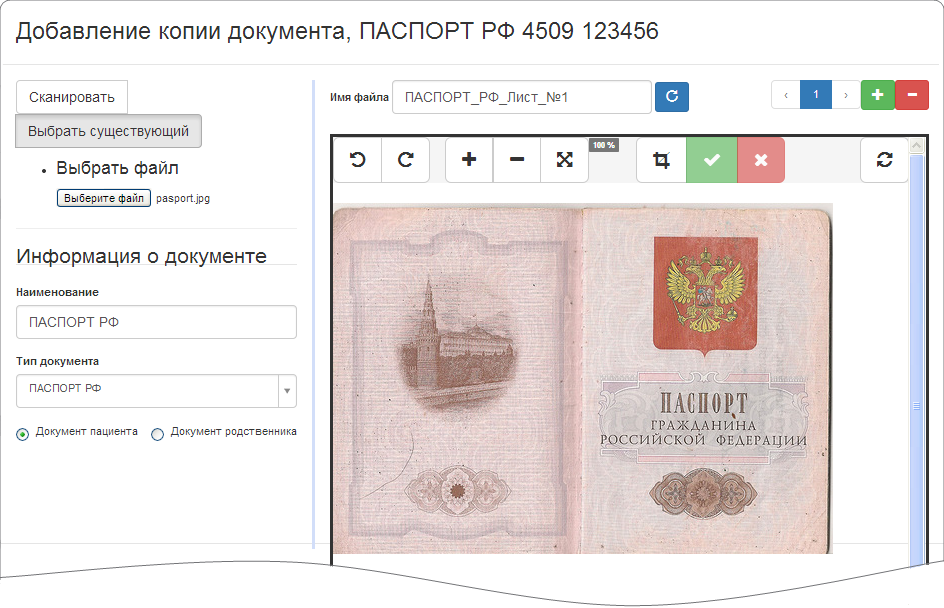
\includegraphics[width = 1\textwidth ,keepaspectratio]{cl_addcopydoc2}
 \caption{Добавление копии документа из файла}
 \label{img_cl_addcopydoc2}
\end{figure} 

Далее следуют заполнить подраздел \dm{Информация о документе} в левой части всплывающего окна:
\begin{itemize}
 \item \dm{Тип документа} -- выбирается из справочника типов документов и должен соответствовать типу прикрепляемого документа.
 \item \dm{Наименование} -- наименование документа, которое будет отображаться в регистрационной карточке пациента. По умолчанию наименование совпадает с выбранным типом документа, но можно ввести произвольное наименование.
 \item Принадлежность прикрепляемого документа выбирается переключателем: документ пациента либо его родственника.
\end{itemize}

В правой части окна находятся следующие управляющие элементы:
\begin{itemize}
 \item \dm{Имя файла} -- имя текущего листа документа. С помощью кнопки 
\includegraphics[scale=0.7]{cpdrefresh} в конце поля можно сформировать автоматическое имя листа.
 \item Кнопки 
\includegraphics[scale=0.7]{cpdadd} и 
\includegraphics[scale=0.7]{cpddel} позволяют добавить и удалить соответственно страницы документа. На каждой странице возможно размещение только одного изображения. При попытке добавить новое изображение на ту же страницу, предыдущее будет удаляться. Таким образом, для сохранения копий нескольких страниц документа, необходимо добавлять соответствующее число страниц. Удаление страницы приводит к удалению размещенного на ней изображения.
 \item Кнопки навигации  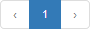
\includegraphics[scale=0.9]{cpdnavi} позволяют перемещаться по страницам документа. Для перемещения можно щелкнуть по номеру страницы либо воспользоваться стралками влево и право для последовательного перехода по страницам. 
\end{itemize}

После внесения всей необходимой информации нужно сохранить ее, нажав кнопку \btn{Сохранить} в правом нижнем углу всплывающего окна. В поле \dm{Копия документа} соответствующего блока регистрационной карточки пациента, а так же в текущем разделе, появится ссылка на прикрепленное изображение (Рисунок \ref{img_cl_addcopydoc3}). Для просмотра и редактирования прикрепленной фотокопии следует щелкнуть по наименованию документа левой кнопкой мыши. 

\begin{figure}[ht]\centering
 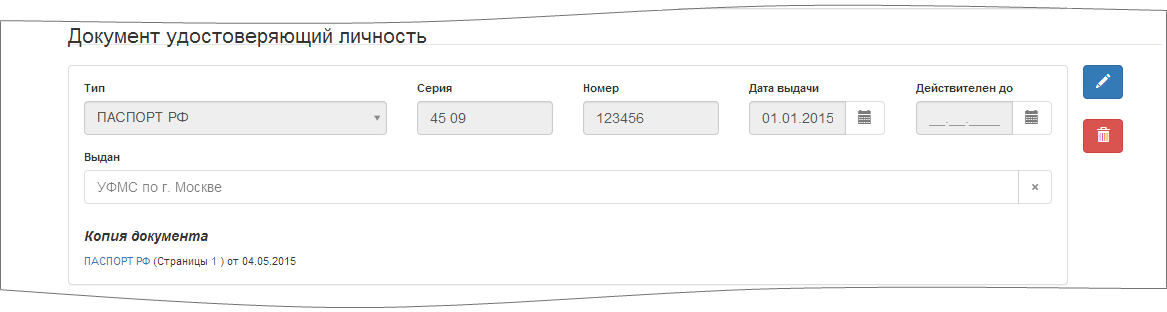
\includegraphics[width = 1\textwidth ,keepaspectratio]{cl_addcopydoc3}
 \caption{Информация о прикреплении копии документа в регистрационной карточке пациента}
 \label{img_cl_addcopydoc3}
\end{figure} 
  

\subsubsection{Блок <<История изменения документов>>} \label{cl_docshistory}

В данном блоке содержится информация обо всех документах, которые когда-либо регистрировались для данного пациента (Рисунок \ref{img_cl_docshistory}). В истории учитываются документы, удостоверяющие личность пациента, полиса ОМС и ДМС, документы, подтверждающие социальные статусы пациента. Для каждого документа указывается его тип, серия, номер, дата начала и окончания действия. Список документов доступен только для просмотра. Редактирование и удаление документов невозможно. 

\begin{figure}[ht]\centering
 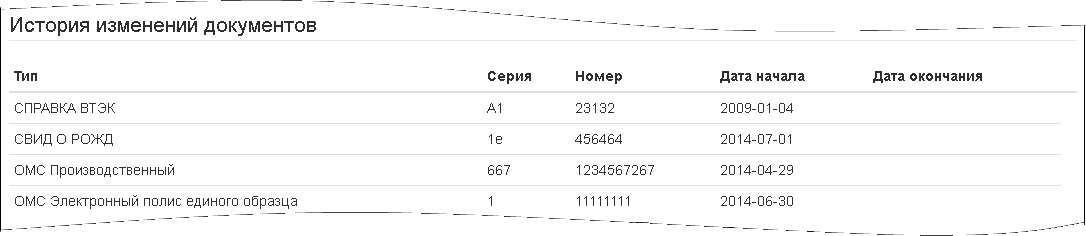
\includegraphics[width = 1\textwidth ,keepaspectratio]{cl_docshistory}
 \caption{Регистрационная карточка пациента. Блок <<История изменений документов>>}
 \label{img_cl_docshistory}
\end{figure} 


\subsection{Регистрация нового пациента} \label{cl_new}

Для регистрации нового пациента необходимо в верхней части страницы нажать кнопку \btn{Обслуживание пациентов}, после чего нажать кнопку \btn{Зарегистрировать пациента}  в правой верхней части открывшейся страницы.

\begin{vnim}
Перед началом регистрации нового пациента необходимо убедиться, что данный пациент не был зарегистрирован ранее. Для этого рекомендуется воспользоваться поиском (см. раздел \ref{cl_find})
\end{vnim}

После нажатия кнопки \btn{Зарегистрировать пациента} откроется страница регистрационной карточки пациента,  содержащая незаполненные поля. Необходимо ввести все данные пациента в пустые поля в соответствии с разделом \ref{cl_card} Для сохранения введенных данных требуется нажать кнопку \btn{Сохранить} в левой части страницы.

Если какие-либо поля регистрационной карточки были заполнены неправильно или некоторые обязательные для заполнения поля остались пустыми, сохранение будет невозможно. В этом случае, при нажатии на кнопку \btn{Сохранить}, рядом с ней появится соответствующая подсказка.

Если сохранение карточки не требуется, нужно нажать кнопку \btn{Отмена} в левой части страницы. Страница регистрации пациента будет закрыта без сохранения данных в БД.

Перемещение между блоками регистрационной карточки можно выполнять как с помощью полос прокрутки или колесика мыши, так и с помощью ссылок на блоки, расположенных в левой части страницы регистрационной карточки пациента (Рисунок \ref{img_cl_content}). Для того, чтобы перейти к нужному блоку с помощью ссылки, достаточно щелкнуть по ней левой кнопкой мыши.

\begin{figure}[ht]\centering
 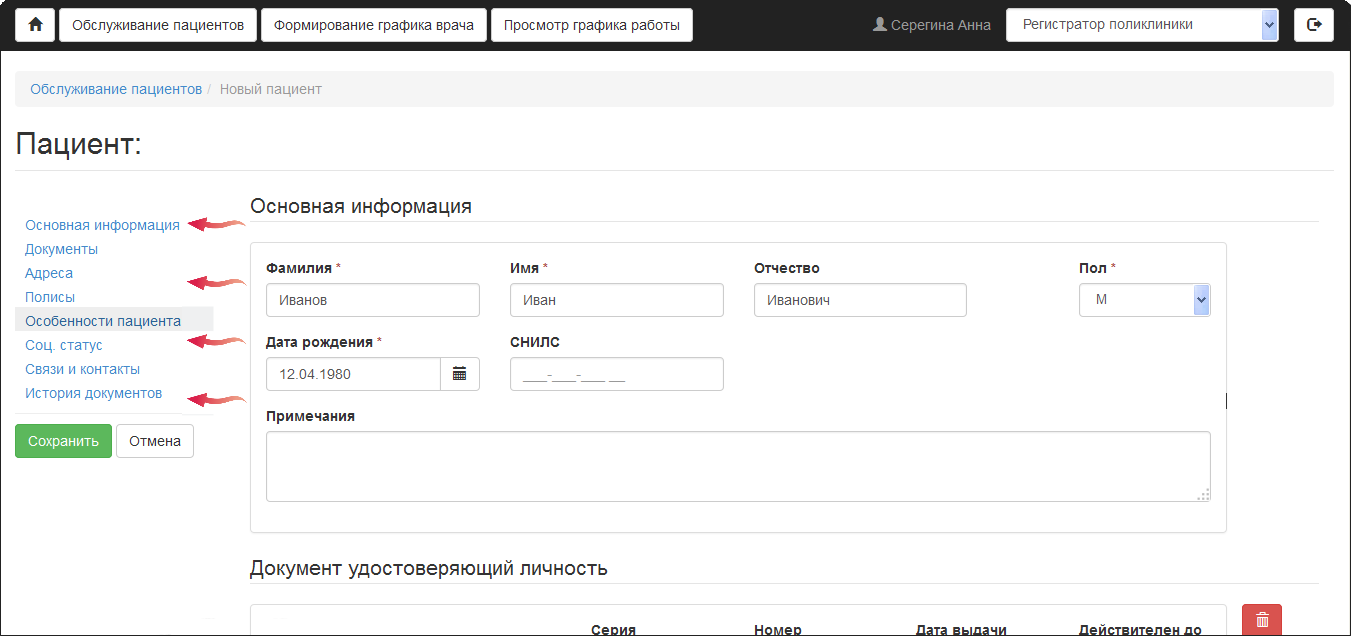
\includegraphics[width = 1\textwidth ,keepaspectratio]{cl_content}
 \caption{Ссылки на блоки регистрационной карточки}
 \label{img_cl_content}
\end{figure} 

\subsection{Редактирование регистрационной карточки пациента}

Данные, введенные в регистрационную карточку пациента, не являются статичными, их можно динамически изменять в соответствии с изменениями и уточнениями персональных данных пациента. При изменении каких-либо документов у пациента, его социального статуса, выявлении новых особенностей и т.п., требуется открыть регистрационную карточку пациента на редактирование и внести в нее соответствующие изменения. 

Для редактирования регистрационной карточки пациента, следует найти пациента в БД (см. раздел \ref{cl_find}), щелкнуть по записи о нем левой кнопкой мыши (Рисунок \ref{img_cl_findrez}) и в появившемся всплывающем окне (Рисунок \ref{img_cl_contrwin}) нажать кнопку \btn{Редактировать данные пациента} или кнопку 
\includegraphics[scale=0.6]{edt} в правом верхнем углу окна. 
}{}

\begin{figure}[ht]\centering
 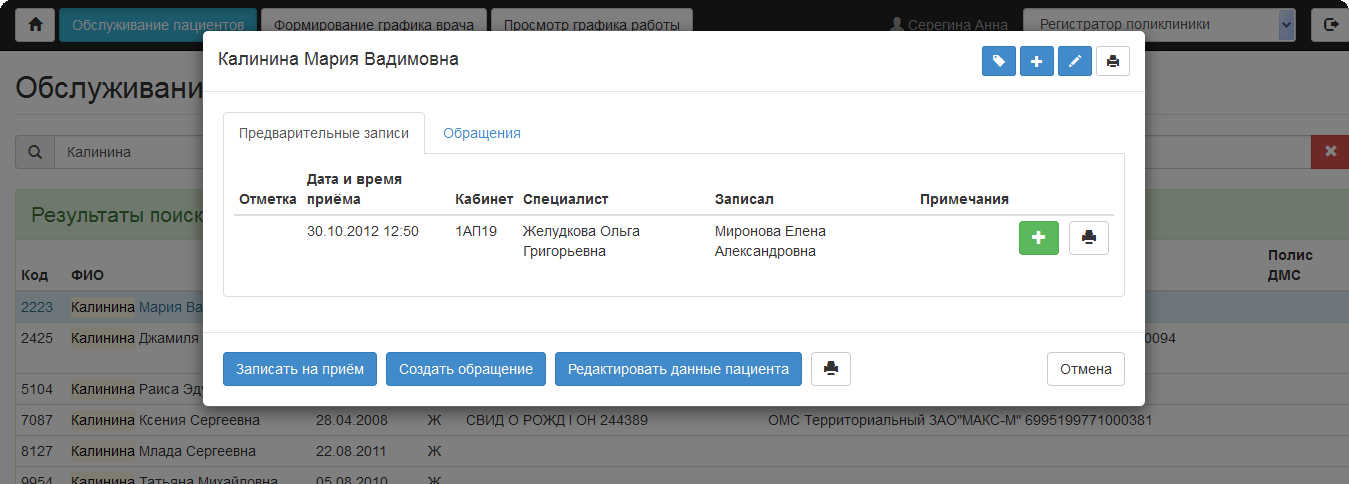
\includegraphics[width = 1\textwidth ,keepaspectratio]{cl_contrwin}
 \caption{Окно управления обслуживанием пациента}
 \label{img_cl_contrwin}
\end{figure} 

\ifthenelse{\isnamedefined{fullversion} \OR \isnamedefined{regversion}}{
Откроется страница, содержащая заполненную регистрационную карточку пациента. Требуется внести изменения в соответствующие поля и сохранить их, нажав кнопку \btn{Сохранить}. Состав полей и методы их заполнения подробно рассмотрены в разделе \ref{cl_card}

Блок основной информации о пациенте доступен для редактирования постоянно. Для того, чтобы отредактировать любой другой блок или подраздел, необходимо нажать кнопку 
\includegraphics[scale=0.6]{edt} справа от него, после чего поля соответствующего блока станут доступными для редактирования.

Для удаления информации из какого-либо блока или подраздела нужно нажать кнопку 
\includegraphics[scale=0.6]{del} справа от  него. Появится диалоговое окно с запросом подтверждения удаления. Следует нажать кнопку \btn{ОК} в этом окне, после чего информация будет удалена. В блоке \dm{Документ удостоверяющий личность} при удалении все поля очищаются, но не удаляются со страницы. При удалении информации в других блоках, поля записи удаляются со страницы.

Кнопка \btn{Добавить новый} в блоках \dm{Адрес регистрации и проживания} и \dm{Медицинские полисы} очищает поля соответствующего подраздела для ввода новых данных. Данные предыдущих полисов при этом сохраняются в истории изменений документов. В остальных разделах данная кнопка создает еще одну запись в выбранном подразделе.

\subsection{Вывод на печать медицинских документов пациента}

Из регистрационной карточки пациента можно распечатать ряд медицинских документов. Для этого требуется нажать кнопку 
\includegraphics[scale=0.6]{print} в правом верхнем углу страницы регистрационной карточки пациента. Откроется окно \dm{Печать документов}, содержащее список доступных печатных форм (Рисунок \ref{img_cl_printm}). Флажками слева от названия отмечаются документы, выбранные для отправки на печать. Нужно снять флажки рядом с названиями документов, печать которых не требуется, и нажать кнопку \btn{Печать}. Отмеченные флажками документы будут выведены на экран для предварительного просмотра и отправлены на принтер.

\begin{figure}[ht]\centering
 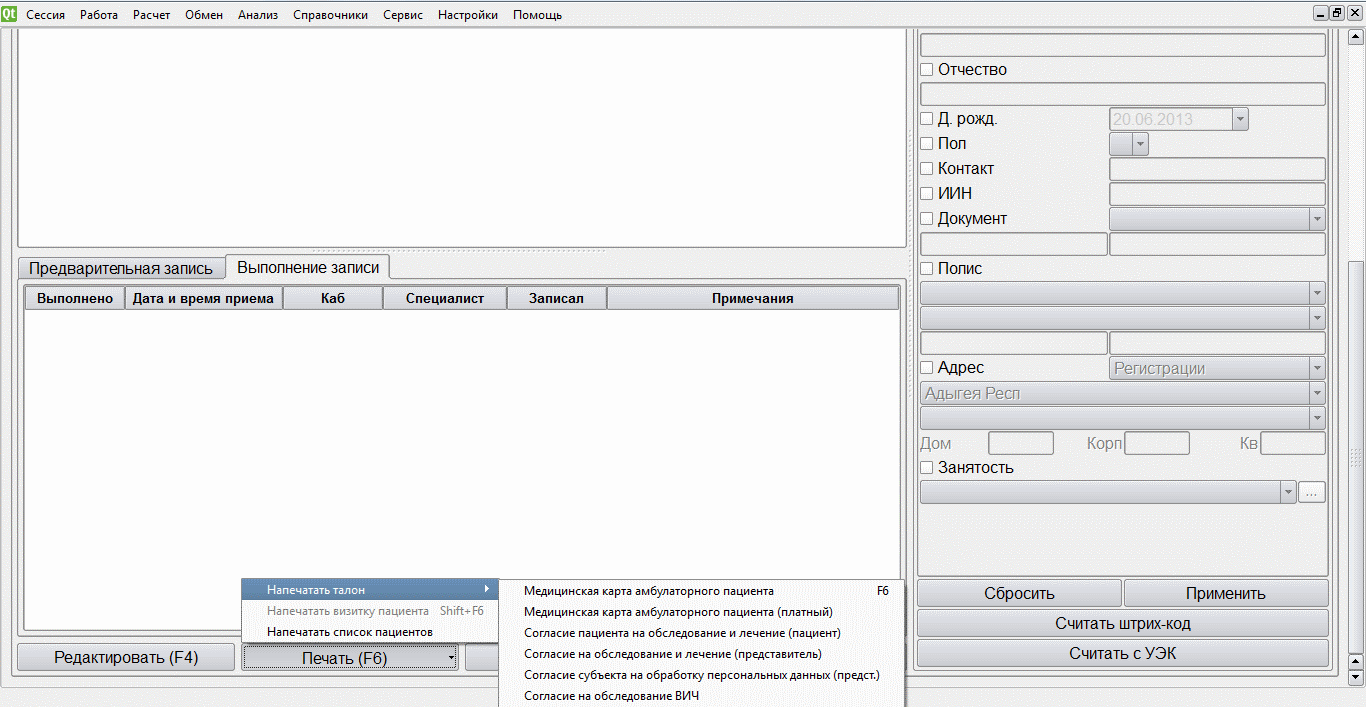
\includegraphics[width = 1\textwidth ,keepaspectratio]{cl_printm}
 \caption{Печать медицинских документов пациента}
 \label{img_cl_printm}
\end{figure} 

Кнопка \btn{Печать компактно} тоже выводит выбранные документы на печать, но не делает переход на новую страницу для каждого нового документа.

Если хотя бы для одного из выбранных для печати документов требуется указане параметров, то в правом нижнем углу всплывающего окна появится кнопка \btn{Далее} (кнопки \btn{Печать} и \btn{Печать компактно}) при этом будут недоступны, при натии на которую осуществляется переход в окно задания параметров формирования печатной формы. После заполнения параметров в данном окне можно нажать кнопку \btn{Печать} и \btn{Печать компактно}.

Печать документов пациента так же можно вызвать со страницы обслуживания пациентов (Рисунок \ref{img_cl_findrez}). Для этого необходимо найти пациента и щелкнуть по нему левой кнопкой мыши. В открывшемся окне (Рисунок \ref{img_cl_contrwin}) нужно нажать кнопку 
\includegraphics[scale=0.6]{print} в нижней части либо в правом верхнем углу окна. Откроется список документов для печати (Рисунок \ref{img_cl_printm}), где можно выбрать и вывести на печать документы вышеописанным способом. 
   
Печать медицинских документов, создаваемых в процессе обследования и лечения пациента, будет рассмотрена в следующих разделах.
}{}
